\documentclass[a4paper, 12pt]{report}
\usepackage{cmap}
\usepackage{amssymb}
\usepackage{amsmath}
\usepackage{graphicx}
\usepackage{amsthm}
\usepackage{upgreek}
\usepackage{setspace}
\usepackage{color}
\usepackage{moreverb}
\usepackage[T2A]{fontenc}
\usepackage[utf8]{inputenc}
\usepackage[normalem]{ulem}
\usepackage{mathtext} % русские буквы в формулах
\usepackage[left=2cm,right=2cm, top=2cm,bottom=2cm,bindingoffset=0cm]{geometry}
\usepackage[english,russian]{babel}
\usepackage[unicode]{hyperref}
\newenvironment{Proof} % имя окружения
{\par\noindent{$\blacklozenge$}} % команды для \begin
{\hfill$\scriptstyle\boxtimes$}
\newcommand{\Rm}{\mathbb{R}}
\newcommand{\Cm}{\mathbb{C}}
\newcommand{\Z}{\mathbb{Z}}
\newcommand{\I}{\mathbb{I}}
\newcommand{\N}{\mathbb{N}}
\newcommand{\rank}{\operatorname{rank}}
\newcommand{\Ra}{\Rightarrow}
\newcommand{\ra}{\rightarrow}
\newcommand{\FI}{\Phi}
\newcommand{\Sp}{\text{Sp}}
\renewcommand{\leq}{\leqslant}
\renewcommand{\geq}{\geqslant}
\renewcommand{\alpha}{\upalpha}
\renewcommand{\beta}{\upbeta}
\renewcommand{\gamma}{\upgamma}
\renewcommand{\delta}{\updelta}
\renewcommand{\varphi}{\upvarphi}
\renewcommand{\phi}{\upvarphi}
\renewcommand{\tau}{\uptau}
\renewcommand{\lambda}{\uplambda}
\renewcommand{\psi}{\uppsi}
\renewcommand{\mu}{\upmu}
\renewcommand{\omega}{\upomega}
\renewcommand{\d}{\partial}
\renewcommand{\xi}{\upxi}
\renewcommand{\epsilon}{\upvarepsilon}
\newcommand{\intx}{\int\limits_{x_0}^x}
\newcommand\Norm[1]{\left\| #1 \right\|}
\newcommand{\sumk}{\sum\limits_{k=0}^\infty}
\newcommand{\sumi}{\sum\limits_{i=0}^\infty}
\newtheorem*{theorem}{Теорема}
\newtheorem*{cor}{Следствие}
\newtheorem*{lem}{Лемма}
\begin{document}
	% Оформление титульного листа
	\begin{titlepage}
		\begin{center}
			\textsc{МИНИСТЕРСТВО ОБРАЗОВАНИЯ РЕСПУБЛИКИ БЕЛАРУСЬ БЕЛОРУССКИЙ ГОСУДАРСТВЕННЫЙ УНИВЕРСИТЕТ
				\\[5mm]
				ФАКУЛЬТЕТ ПРИКЛАДНОЙ МАТЕМАТИКИ И ИНФОРМАТИКИ\\[2mm]
				Кафедра компьютерных технологий и систем
			}
			
			\vfill
			
			\textbf{Отчет по лабораторной работе №2\\
				«Решение смешанных задач для уравнения теплопроводности»\\
				Вариант 4
				\\[26mm]
			}
		\end{center}
		
		\hfill
		\begin{minipage}{.5\textwidth}
			\begin{flushright}
				Гут Валерии Александровны\\
				студентки 3 курса\\
				специальности «прикладная математика»\\[5mm]
				
				Преподаватель:\\[2mm] 
				И. С. Козловская\\
			\end{flushright}
		\end{minipage}%
		\vfill
		\begin{center}
			Минск, 2024\ г.
		\end{center}
	\end{titlepage}
	\newpage
	\section*{Постановка задачи}
	Решить следующую смешанную задачу 
	\begin{equation}
		\begin{cases}
		u_t - a^2 u_{xx} = \dfrac{1}{1+x},\\
		u_x|_{x=0} = 0,\\
		u|_{x=l} = 0,\\
		u|_{t=0} = 0.
	\end{cases}
	\end{equation}
	\section*{Решение задачи в пакете Wolfram Mathematica}
	Перепишем данную задачу в Wolfram Mathematica
	$$
		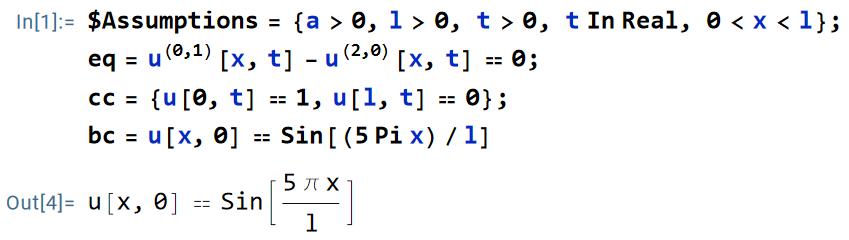
\includegraphics[scale=0.5]{images/img1}
	$$
	Так как уравнение в задаче (1) является неоднородным, то решение мы будем искать в виде суммы
	\begin{eqnarray}
		u(x,t) = \sum_{n=0}^{\infty} T_n(t)X_n(x).
	\end{eqnarray}
	Составим задачу Штурма-Ливувилля для соответствующего однородного уравнения \begin{eqnarray}
	\begin{cases}
	X''(x) + \lambda^2 X(x) = 0,\\
	X'(0) = 0,\\
	X(l) = 0.
	\end{cases}
	\end{eqnarray}
	Найдем решение этой задачи в Wolfram Mathematica
	$$
		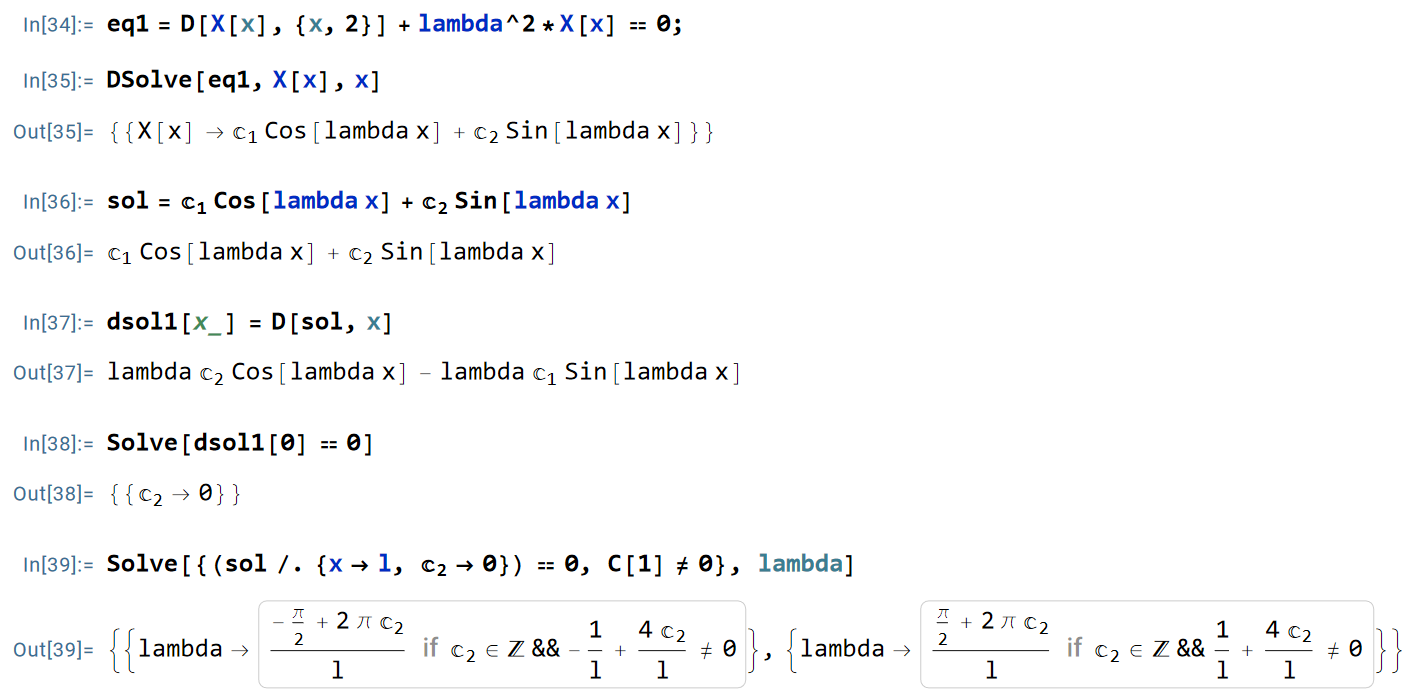
\includegraphics[scale=0.45]{images/img2}
	$$
	То есть
	$$
		X(x) = C_1\cos \lambda x + C_2 \sin \lambda x.
	$$
	И поскольку $\lambda > 0$, то $C_2 = 0$. А так как $C_1 \ne 0$, то а значит $$\lambda_n = \dfrac{\pi + 2\pi n}{2l},\quad X_n(x) = \cos \dfrac{\pi + 2\pi n}{2l} x, \quad n = 0,1,\ldots.$$
	Подставим $X_n(x)$ в (2) и получим \begin{equation}
		u(x,t) = \sum_{n=0}^{\infty} T_n(t)  \cos \dfrac{\pi + 2\pi n}{2l} x.
	\end{equation}
	Чтобы определить вид функций $T_n(t)$, подставим решение в виде (4) в уравнение задачи (1)
	$$\sum_{n=0}^\infty T'_n(t) \cos \dfrac{\pi + 2\pi n}{2l} x + a^2 \sum_{n=0}^\infty T_n(t) \left(\cos \dfrac{\pi + 2\pi n}{2l}\right)^2 \cos \dfrac{\pi + 2\pi n}{2l} x = \dfrac{1}{1+x}.$$
	Разложим правую часть равенства в ряд Фурье по собственным функциям:
	$$\dfrac{1}{1+x} = \sum_{n=0}^\infty f_n \cos \dfrac{\pi + 2\pi n}{2l} x,$$
	$$f_n = \dfrac2l \int\limits_0^l\dfrac{1}{1+x}\cos \dfrac{\pi + 2\pi n}{2l} x dx.$$
	Этот интеграл неберущийся, в явном виде первообразную мы не сможем найти. Поэтому будем далее под обозначением $f_n$ иметь значение этого интеграла. В Wolfram Mathematica можно получить следующий результат
	$$
		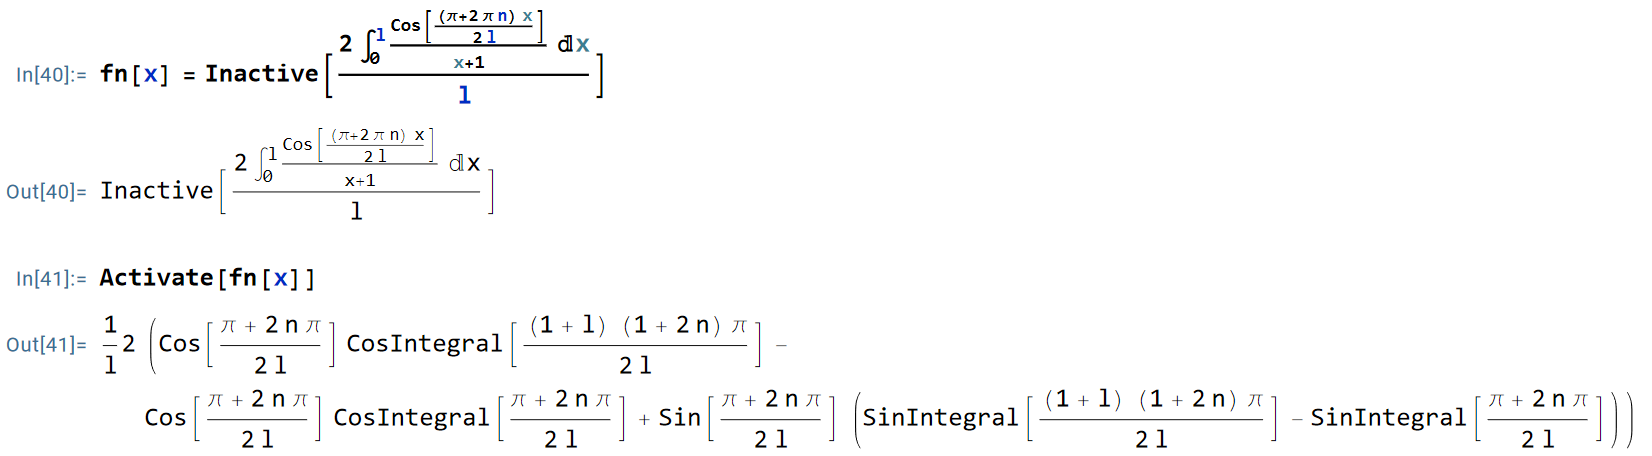
\includegraphics[scale=0.40]{images/img3}
	$$
	
	Таким образом, получаем
	\begin{multline*}
		\sum_{n=0}^\infty T'_n(t) \cos \dfrac{\pi + 2\pi n}{2l} x + \sum_{n=0}^\infty T_n(t) \left(a\dfrac{\pi + 2\pi n}{2l}\right)^2 \cos \dfrac{\pi + 2\pi n}{2l} x = \sum_{n=0}^\infty f_n \cos \dfrac{\pi + 2\pi n}{2l} x.
	\end{multline*}
	Отсюда, приравнивая коэффициенты при рядах, получаем
	\begin{equation}
		T'_n(t) + \left(a\dfrac{\pi + 2\pi n}{2l}\right)^2 T_n(t) = f_n.
	\end{equation}
	Подставляя в (4) начальное условие задачи (1), получаем
	\begin{equation}
		\sum_{n=0}^{\infty} T_n(0)  \cos \dfrac{\pi + 2\pi n}{2l} x = 0 \Rightarrow T_n(0) = 0.
	\end{equation}
	Решение задачи Коши (5), (6) найдем с помощью Wolfram Mathematica. Сперва построим общее решение уравнения (5)
	$$
		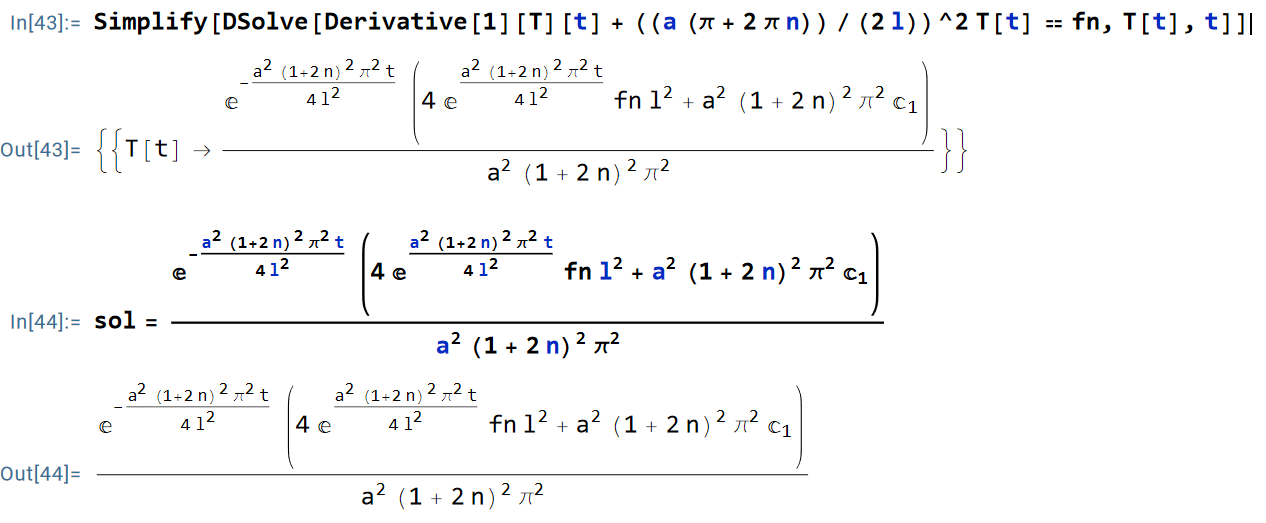
\includegraphics[scale=0.45]{images/img4}
	$$
	то есть 
	\begin{equation}
		T_n(t)=\dfrac{1}{a^2(\pi + 2\pi n)^2}e^{-\frac{a^2(\pi + 2\pi n)^2t}{4l^2}}\left(4e^{\frac{a^2(\pi + 2\pi n)^2t}{4l^2}} f_n l^2 +a^2(\pi + 2\pi n)^2 C_1 \right).
	\end{equation}
	Используя начальное условие (6), находим значение $C_1$
	$$
		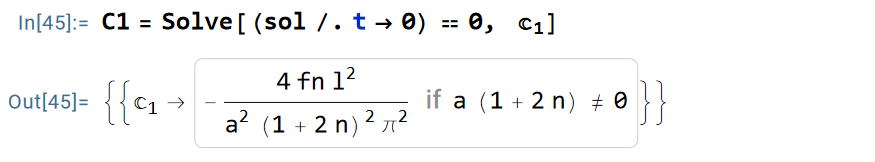
\includegraphics[scale=0.5]{images/img5}
	$$
	то есть \begin{equation}
		C_1 = -\dfrac{4 f_n l^2}{a^2(\pi + 2\pi n)^2}.
	\end{equation}
	Подставим это значение в (7) и получим вид функций $T_n(t)$
	$$
		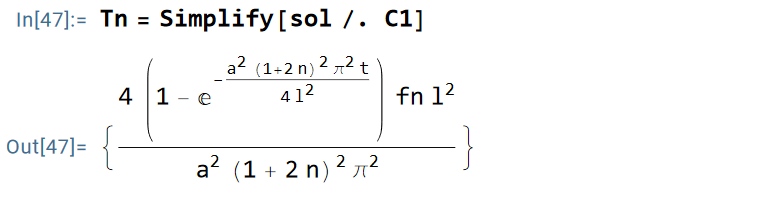
\includegraphics[scale=0.5]{images/img6}
	$$
	то есть
	\begin{equation}
		T_n(t)=\dfrac{4 f_n l^2}{a^2(\pi + 2\pi n)^2}\left(1-e^{-\frac{a^2(\pi + 2\pi n)^2t}{4l^2}}\right).
	\end{equation}
	Тогда $n$-ый член суммы (2), которая является решением, можно записать как
	$$
		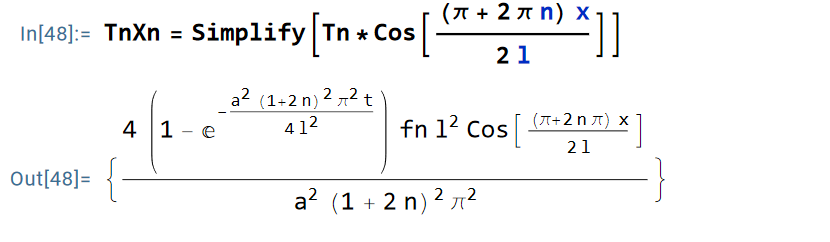
\includegraphics[scale=0.5]{images/img7}
	$$
	то есть 
	\begin{equation}
		T_n(t)X_n(x) = \dfrac{4 f_n l^2}{a^2(\pi + 2\pi n)^2}\left(1-e^{-\frac{a^2(\pi + 2\pi n)^2t}{4l^2}}\right)\cos \left(\dfrac{\pi + 2\pi n}{2l}x\right).
	\end{equation}
	Для проверки подставим данный коэффициент в задачу (1)
	$$
		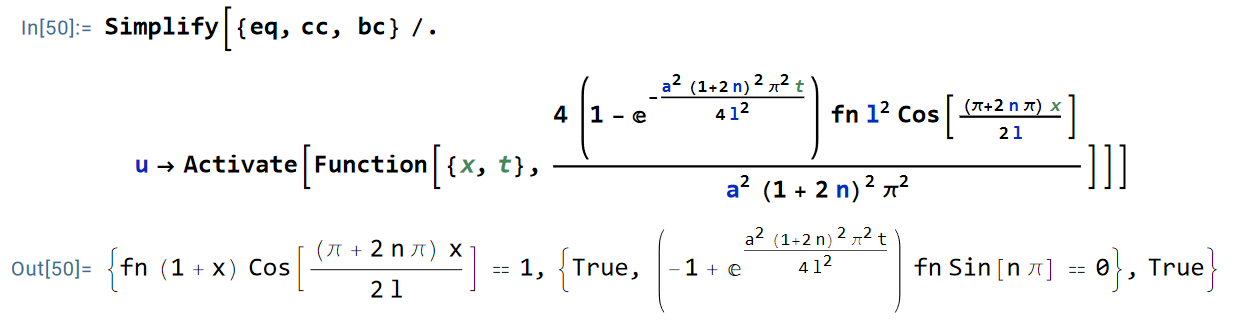
\includegraphics[scale=0.5]{images/img8}
	$$
	то есть $T_n(t)X_n(x)$ удовлетворяют всем дополнительным условиям (второе условие также выполнено, так как $\sin \pi n = 0$). Эти функции также удовлетворяют и самому уравнению, так как мы получили равенство $$f_n\cos \left(\dfrac{\pi + 2\pi n}{2l}x\right)=\dfrac{1}{1+x},$$
	а значение слева и является $n$-ым членом разложения в ряд Фурье правой функции по степеням собственных функций.\\\\
	Таким образом, решение задачи (1) задано функцией
	\begin{equation}
		u(x,t) = \sum_{n=0}^\infty\dfrac{4 f_n l^2}{a^2(\pi + 2\pi n)^2}\left(1-e^{-\frac{a^2(\pi + 2\pi n)^2t}{4l^2}}\right)\cos \left(\dfrac{\pi + 2\pi n}{2l}x\right).
	\end{equation}
	Теперь найдем решение задачи (1) альтернативным образом через команду DSolve
	$$
		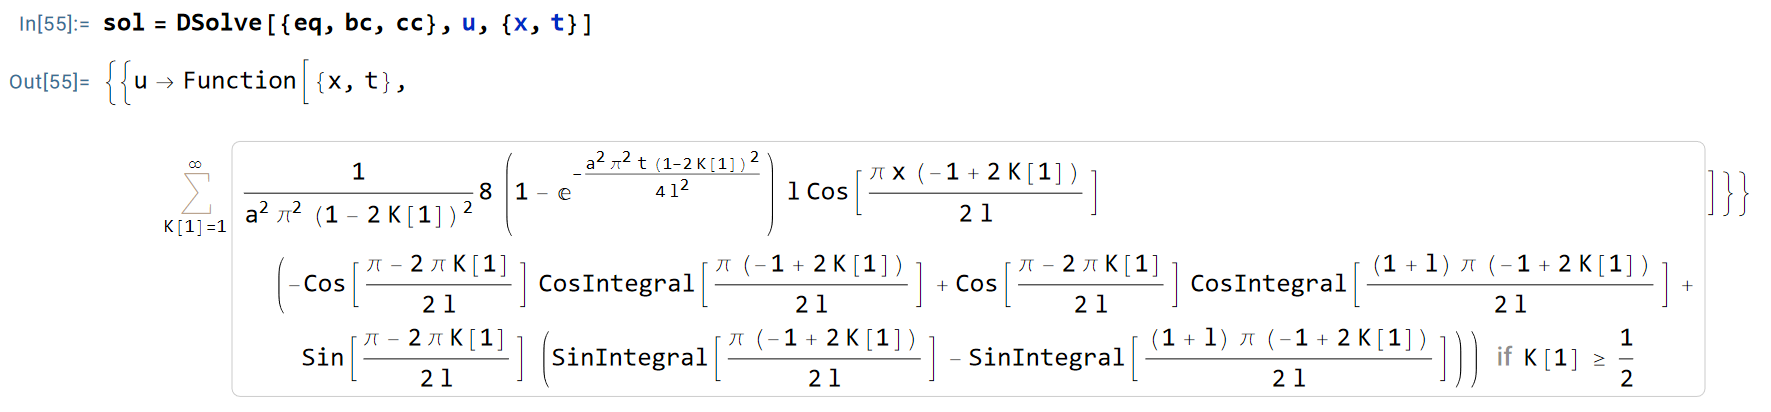
\includegraphics[scale=0.4]{images/img10}
	$$
	что совпадает с построенным нами решением, если в нем расписать $f_n$.
	\section*{Визуализация решения с помощью Wolfram Mathematica}
	Рассмотрим дополнительные условия задачи (1). Из физического смысла начальное условие задает температуру стержня в каждом сечении $x$ в начальный момент времени $t = 0$, следовательно в момент
	$t = 0$ температура $u$ в каждом сечении стрежня нулевая. Граничное условие первого рода задает температуру $u=0$ на конце стрежня $x=l$. Граничное условие второго рода заключается в том, что на конец стрежня $x=0$ подается заданный тепловой поток $u=0$. Таким образом, на одном конце
	стержня поддерживается температура в 0 градусов, а на второй конец стержня подается
	тепловой поток в 0 градусов.
	Построенное решение задачи колеблется около 0 и сходится в 0. Из-за этого, если пытаться строить график теплообмена, то он бы не мог учитывать такие малые изменения по температуре.
\section*{Вывод}
Таким образом, мы нашли решение смешанной задачи для уравнения теплопроводности методом разделения переменных, а затем проверили, правильно ли оно было вычислено, с помощью Wolfram Mathematica.
\end{document}

 